\documentclass[12pt]{article}
%\usepackage{geometry}                % See geometry.pdf to learn the layout options. There are lots.
%\geometry{letterpaper}                   % ... or a4paper or a5paper or ... 
%\geometry{landscape}                % Activate for for rotated page geometry
\usepackage[parfill]{parskip}    % Activate to begin paragraphs with an empty line rather than an indent
\usepackage{daves,fancyhdr,natbib,graphicx,dcolumn,amsmath,lastpage,url}
\usepackage{multicol}
\usepackage{amsmath,amssymb,epstopdf,longtable}
\usepackage[final]{pdfpages}
\usepackage{booktabs}

\DeclareGraphicsRule{.tif}{png}{.png}{`convert #1 `dirname #1`/`basename #1 .tif`.png}
\pagestyle{fancy}
\lhead{CE 5362 Surface Water Modeling}
\rhead{SPRING 2020}
\lfoot{}
\cfoot{}
\rfoot{Page \thepage\ of \pageref{LastPage}}
\renewcommand\headrulewidth{0pt}


\setcounter{MaxMatrixCols}{20}

%%%%%%%%%% Will's listing environment %%%%%%%
\usepackage[left=1.25in, right=1.25in,
            top=1in, bottom=1in]{geometry}                % See geometry.pdf to learn the layout options. There are lots.
\geometry{letterpaper}

\usepackage{ragged2e}

\usepackage{xcolor}
\newcommand{\codeRcolor}{0.93}
\newcommand{\codeGcolor}{0.93}
\newcommand{\codeBcolor}{0.93}
\definecolor{lightgrey}{rgb}{\codeRcolor,
                             \codeGcolor,
                             \codeBcolor}

\newcommand{\listingfont}{\fontsize{7pt}{8pt}\selectfont\ttfamily}
\usepackage{listings}
\lstset{basicstyle = \listingfont,
        breaklines = true,
        frame=tb,
        xleftmargin=12pt,
        framexleftmargin=6pt,
        framexrightmargin=6pt,
        xrightmargin=12pt,
        columns=fixed}
\lstset{lineskip=-1pt}
\lstset{backgroundcolor=\color{lightgrey}}


\usepackage[font={footnotesize},
            labelfont={sf,bf},
            textfont={sf},
            singlelinecheck=false,
            labelsep=none,
            justification=RaggedRight,
            aboveskip=0pt,
            belowskip=7pt plus 1pt minus 1pt,
            textformat=period]{caption}
\DeclareCaptionLabelSeparator{mystyle}{.\quad}
\captionsetup{labelsep=mystyle}
%%%%%%%%% End Will's listing environment ABOVE %%%%%%%%%

\begin{document}
\begingroup
\begin{center}
{\textbf{{CE 5362 Surface Water Modeling \\ Lesson 5}}}
\end{center}

\begin{center}
by \\
Theodore G. Cleveland \\%and Caroline M. Neale\\
Department of Civil, Environmental, and Construction Engineering\\
Texas Tech University\\
\end{center}

\begin{figure}[h!] %  figure placement: here, top, bottom, or page
\centering
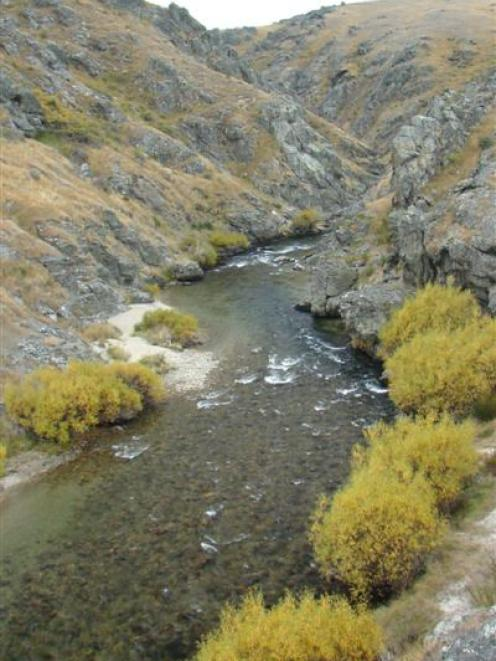
\includegraphics[height=5in]{the_nevis_river_photo_supplied__1234583207.jpg} 
\end{figure}

\endgroup
\tableofcontents
%%%%%%%%%%%%%%%%%%%%%%%%%%%%%%%%%%%%%%%
%%%%%%%%%%%%% CHAPTER 7 %%%%%%%%%%%%%%%%%%%%%%%%%%%%%%%%%%
%%%%%%%%%%%%%% Numerical Integration %%%%%%%%%%%%%%%%%%%%%%%%%%%%%
%%%%%%%%%%%%%%%%%%%%%%%%%%%%%%%%%%%%%%%%%%%%%%%%%%%%%%%
\section{Open Channel Flow}
This chapter derives the St. Venant equations for one-dimensional (1-D) open channel flow.   
The equations were originally developed in the 1850's, so the concept is not very new.  
The tools have changed since that time; computational methods have greatly increased the utility of these equations.
\subsection{St. Venant Equations}
%%%%%%%%%%%%%%%%%%%%%%%%%%
In general, 1-D unsteady flow would be considered state-of-practice computation; every engineer would be expected to be able to make such calculations (albeit using software).  
2-D computation is becoming routine using general purpose software.  
3-D computation as of this writing (circa 2009) is still in the realm of state-of-art, and would not be within the  capability a typical consulting firm.

The conservation of mass, momentum, and energy in the context of the cell balance method is used to develop the mathematical and computational structure.  
The cell balance is a computational structure that is analogous to the Reynolds transport theorem, except the end result are difference equations that can be updates to approximate physical processes.  
We later employ the method for porous media flow.
The philosophy is a hybrid approach -- instead of developing the  differential equations first, then numerical approximations, the numerical constructs are built directly and the limiting process is employed to demonstrate that the constructs indeed mimic the differential equations that describe our current understanding of the physics.  

\subsubsection{The Computational Cell}
The cell balance method envisions the world as representable by a computational cell (or more typically a collection of cells) with some finite dimension, fixed in space about a cell centroid.  Some dimensions are changeable -- such as depth.\footnote{This concept is distinct from a particle view of the world, which will be explored in future versions of this course.}  

The fundamental computational element is a computational cell or a reach.\footnote{Some professional software, in particular HEC-RAS, considers a reach to be a specific portion of a river system that may be comprised of several computational sub-reaches (cells).  The engineer will need to consider the context and the tool used to decide which way to describe their problem --- and it is quite possible that the author of this document may be wrong in terminology!}
Figure \ref{fig:reach_sketch} is a sketch of a portion of a channel.  The left-most section is uphill (and upstream) of the right-most section.
The section geometry is arbitrary, but is drawn to look like a channel cross section.

The length of the reach (distance between each section along the flow path) is $\Delta x$.  The depth of liquid in the section is $z$, the width at the free surface is $B(z)$, the functional relationship established by the channel geometry.  
The flow into the reach on the upstream face is $Q-\frac{\partial Q}{\partial x}*\frac{\Delta x}{2}$.  The flow out of  the reach on the downstream face is $Q+\frac{\partial Q}{\partial x}*\frac{\Delta x}{2}$.  The direction is strictly a sign convention and the development does not require flow in a single direction.  The topographic slope is $S_0$, assumed relatively constant in each reach, but can vary between reaches.  



%Figure \ref{fig:single_cell} is a sketch that illustrates a single computational cell. Within the cell's volume average properties of the world which we are trying to simulate are represented.  In the context of flow these properties would be head, storage within the cell, fluid density, constituent concentration, etc.   Intensive or extensive properties related to these average properties enter and leave the cell through flux terms ($J_{x+-{\partial x}/2} $)at the cell boundaries.   The cell's volume is the product of the cell dimensions ($\Delta x \times \Delta y \times \Delta z$).  In some situations the volume is allowed to change, in others it is held fixed.  It is the modeler's choice of how to handle the dimensional fixation\footnote{In many surface flow problems, $\Delta z$ is a variable and only the width and length are fixed.  The backwater curves already presented implicitly used this structure.} or lack of fixation.

\begin{figure}[h!] %  figure placement: here, top, bottom, or page
   \centering
   \includegraphics[width=5in]{reach_sketch.jpg} 
   \caption{Reach/Computational Cell}
   \label{fig:reach_sketch}
\end{figure}

\subsubsection{Assumptions}
The development of the unsteady flow equations in this chapter uses several assumptions:
\begin{enumerate}
\item The pressure distribution at any section is hydrostatic --- this assumption allows computation of pressure force as a function of depth.
\item Wavelengths are long relative to flow depth --- this is called the shallow wave theory.
\item Channel slopes are small enough so that the topographic slope is roughly equal to the tangent of the angle formed by the channel bottom and the horizontal. 
\item The flow is one-dimensional --- this assumption implies that longitudinal dimension is large relative to cross sectional dimension.  Generally river flows will meet this assumption, it fails in estuaries where the spatial dimensions (length and width) are roughly equal.  Thus rivers that are hundreds of feet wide imply that reaches are miles long.  If this assumption cannot be met, then 2-D methods are more appropriate.
\item Friction is modeled by Chezy or Manning's type empirical models.  The particular friction model does not really matter, but historically these equations have used the friction slope concept as computed from one of these empirical models.
\end{enumerate}

The tools that are used to build the equations are conservation of mass and linear momentum.
%The flux terms convey mass into the cell (conservation of mass), or momentum (conservation of momentum; linear and angular), or energy (conservation of energy).  In many problems momentum and energy look the same (from a computational point of view), but are fundamentally different concepts although related through the friction term in the momentum equation.

%These flux terms are generally related to the average properties in the adjacent cells and hence this (adjacent interactions) relationship is how the flux terms are determined and in turn how the average properties are updated.

\subsubsection{Conservation of Mass}
The conservation of mass in the cell is the statement that mass entering and leaving the cell is balanced by the accumulation or lass of mass within the cell.   For pedagogical clarity, this section goes through each part of a mass balance then assembles into a difference equation of interest.    

\textsl{Mass Entering:}  Mass enters from the left of the cell in our sketch.  This direction only establishes a direction convention and negative flux means the arrow points in the direction opposite of that in the sketch.  In the notation of the sketch mass entering in a short time interval is:


\begin{equation}
\dot{M}_{in}= \rho * ( Q-\frac{\partial Q}{\partial x}*\frac{\Delta x}{2})*\Delta t
\end{equation}

where $\rho$ is the fluid density.  Notice that the mass flux is evaluated at the cell interface and not the centroid, while by convention $\rho$ is assumed to be defined as an average cell property.

\textsl{Mass Leaving:}  Mass leaves from the right of the cell in our sketch.    In the notation of the sketch mass leaving is:

\begin{equation}
\dot{M}_{out}= \rho * ( Q+\frac{\partial Q}{\partial x}*\frac{\Delta x}{2})*\Delta t
\end{equation}

\textsl{Mass Accumulating:}  Mass accumulating within the reach is stored in the prism depicted in the sketch by the dashed lines.  The product of density and prism volume is the mass added to (or removed from) storage.  

The rise in water surface in a short time interval is $\frac{\partial z}{\partial t}*\Delta t$.
The plan view area of the prism is $B(z)* \Delta x$.
The product of these two terms is the mass added to storage, expressed as:

\begin{equation}
\dot{M}_{storage} = \rho *( \frac{\partial z}{\partial t}*\Delta t) *B(z)* \Delta x 
\end{equation}

Equating the accumulation to the net inflow produces 

\begin{equation}
 \rho *( \frac{\partial z}{\partial t}*\Delta t) *B(z)* \Delta x =  \rho * ( Q-\frac{\partial Q}{\partial x}*\frac{\Delta x}{2})*\Delta t - \rho * ( Q+\frac{\partial Q}{\partial x}*\frac{\Delta x}{2})*\Delta t
\end{equation}

This is the mass balance equation for the reach.  If the flow is isothermal, and essentially incompressible then the density is a constant and can be removed from both sides of the equation.  

\begin{equation}
( \frac{\partial z}{\partial t}*\Delta t) *B(z)* \Delta x =  ( Q-\frac{\partial Q}{\partial x}*\frac{\Delta x}{2})*\Delta t - ( Q+\frac{\partial Q}{\partial x}*\frac{\Delta x}{2})*\Delta t
\end{equation}

Rearranging the right hand side produces

\begin{equation}
( \frac{\partial z}{\partial t}*\Delta t) *B(z)* \Delta x =  -\frac{\partial Q}{\partial x}*\frac{\Delta x}{2}*\Delta t - \frac{\partial Q}{\partial x}*\frac{\Delta x}{2}*\Delta t = -\frac{\partial Q}{\partial x}*\Delta x*\Delta t
\end{equation}

Dividing both sides by $\Delta x*\Delta t$ yields

\begin{equation}
( \frac{\partial z}{\partial t}) *B(z) = -\frac{\partial Q}{\partial x}
\end{equation}

This equation is the conventional representation of the conservation of mass in 1-D open channel flow.   If the equation includes lateral inflow the equation is adjusted to include this additional mass term.  The usual lateral inflow is treated as a discharge per unit length added into the mass balance as expressed in Equation \ref{eqn:continunity}.

\begin{equation}
( \frac{\partial z}{\partial t}) *B(z) + \frac{\partial Q}{\partial x} = q
\label{eqn:continunity}
\end{equation}

This last equation is one of the two equations that comprise the St. Venant equations.  The other equation is developed from the conservation of linear momentum --- the next section.

\subsubsection{Conservation of Momentum}
The conservation of momentum is the statement of the change in momentum in the reach is equal to the net momentum entering the reach plus the sum of the forces on the water in the reach.  As in the mass balance, each component will be considered separately for pedagogical clarity.

Figure \ref{fig:motion_sketch} is a sketch of the reach element under consideration, on some non-zero sloped surface.  
\begin{figure}[h!] %  figure placement: here, top, bottom, or page
   \centering
   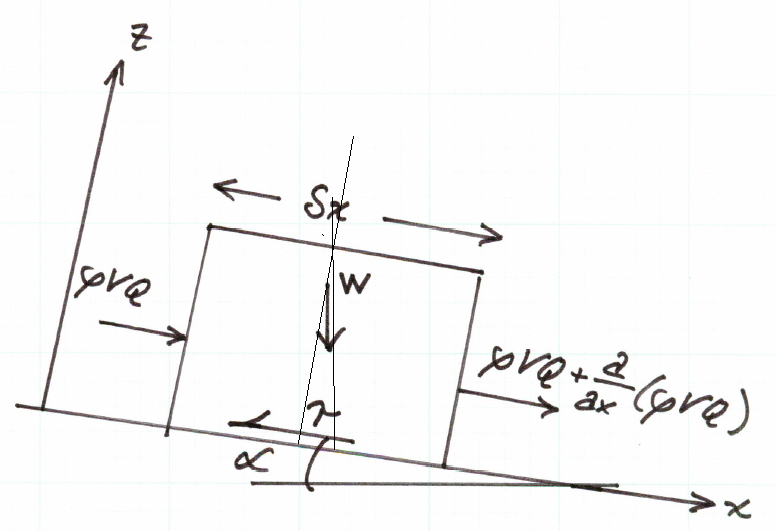
\includegraphics[width=5in]{motion_sketch1.jpg} 
   \caption{Equation of motion definition sketch}
   \label{fig:motion_sketch}
\end{figure}

\textsl{Momentum Entering:} 
Momentum entering on the left side of the sketch is 

\begin{equation}
\rho*QV = \rho*V^2A
\end{equation}


\textsl{Momentum Leaving:} 
Momentum leaving on the right side of the sketch is 

\begin{equation}
\rho*QV+\frac{\partial}{\partial x}(\rho*QV)\delta x = \rho*V^2A+\frac{\partial}{\partial x}(\rho*V^2A)\delta x
\end{equation}

\textsl{Momentum Accumulating:}
The momentum accumulating is the rate of change of linear momentum:
\begin{equation}
\frac{dL}{dt}= \frac{d~(mV)}{dt}=\frac{\partial}{\partial t}(\rho*AV*\delta x)=\rho*\delta x\frac{\partial}{\partial t}(AV)
\end{equation}


\textsl{Forces on the liquid in the reach:}

\textsl{Gravity forces:}  The gravitational force on the element is the product of the mass in the element and the downslope component of acceleration.

The mass in the element is $\rho*A\delta x$ 

The $x$-component of acceleration is $g~sin(\alpha)$, which is $\approx~S_0$ for small values of $\alpha$.

The resulting force of gravity is is the product of these two values:

\begin{equation}
F_g=\rho g *AS_0~\delta x
\end{equation}



\textsl{Friction forces:}   Friction force is the product of the shear stress and the contact area.  In the reach the contact area is the product of the reach length and average wetted perimeter.  

\begin{equation}
F_{fr} = \tau * P_w * \delta x
\end{equation}

where $P_w = A/R$, $R$ is the hydraulic radius.  A good approximation for shear stress in unsteady flow is $\tau = \rho g R S_f$.  $S_f$ is the slope of the energy grade line at some instant and is also called the friction slope.  This slope can be empirically determined by a variety of models, typically Chezy's or Manning's equation is used.  In either of these two models, we are using a STEADY FLOW equation of motion to mimic unsteady behavior --- nothing wrong, and it is common practice, but this decision does limit the frequency response of the model (the ability to change fast --- hence the shallow wave theory assumption!).

The resulting friction model is

\begin{equation}
F_{fr} =  \rho g A S_f * \delta x
\end{equation}


\textsl{Pressure forces:}   
[Set the equations, backfill discussion next version]

\begin{equation}
F_p = \int_{A} {dF}
\end{equation}

\begin{figure}[h!] %  figure placement: here, top, bottom, or page
   \centering
   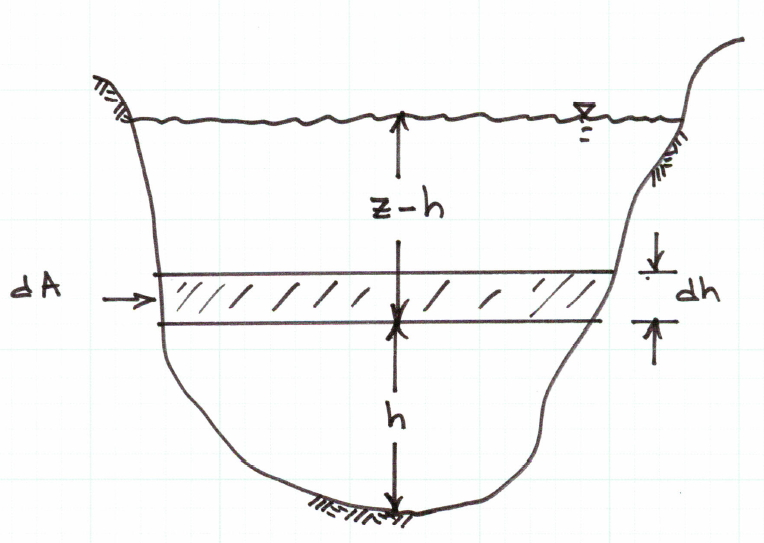
\includegraphics[width=5in]{pressure_sketch.jpg} 
   \caption{Pressure integral sketch}
   \label{fig:pressure_sketch}
\end{figure}

\begin{equation}
dF = (z-h)\rho g \xi (h) dh
\end{equation}

where $\xi (h)$ is the width of the panel at a given distance above the channel bottom ($h$) at any section.

\begin{equation}
F_{p~net} = F_{p~up} - F_{p~down}
\end{equation}

\begin{equation}
F_{p~net} = F_p -( F_p + \frac{\partial F_p}{\partial x}*\delta x) = - \frac{\partial F_p}{\partial x}*\delta x
\end{equation}

\begin{equation}
 - \frac{\partial F_p}{\partial x}*\delta x = -\frac{\partial}{\partial x}[\int_{0}^{Z}\rho g (z-h) \xi(h) dh ] \delta x
\end{equation}

\begin{equation}
F_{p~net}  = -\rho g [\frac{\partial z}{\partial x}\int_{0}^{Z} \xi(h) dh + \int_{0}^{Z} (z-h) \xi(h) \frac{\partial \xi(h)}{\partial x} dh] \delta x
\end{equation}

The first term integrates to the cross sectional area, the second term is the variation in pressure with position along the channel.

The other pressure force to consider is the bank force (the pressure force exerted by the banks on the element).  This force is computed using the same type of integral structure except the order is swapped.

\begin{equation}
F_{p~bank} =  [\int_{0}^{Z} \rho g (z-h) \frac{\partial \xi(h)}{\partial x} \delta x] dh
\end{equation}

Now we put everything together.

\begin{equation}
{Momentum}_{in}-{Momentum}_{out} + \sum{F} = \frac{d(mV)}{dt}
\end{equation}

Substitution of the pieces:

\begin{equation}
{Momentum}_{in}-{Momentum}_{out} + F_{p~net}+F_{bank} + F_{gravity} - F_{friction}  = \frac{d(mV)}{dt}
\end{equation}

Now when the expressions for each expressions for each part

\begin{equation}
\begin{split}
\rho*V^2A- \rho*V^2A-\frac{\partial}{\partial x}(\rho*V^2A)\delta x  \\
-\rho g \frac{\partial z}{\partial x}\int_{0}^{Z} \xi(h) dh \delta x
- [\int_{0}^{Z}\rho g (z-h)  \frac{\partial \xi(h)}{\partial x} dh] \delta x \\ 
+[\int_{0}^{Z} \rho g (z-h) \frac{\partial \xi(h)}{\partial x} \delta x] dh\\
+\rho g *AS_0~\delta x \\- (\rho g R S_f * \delta x)  \\ =  \rho*\delta x\frac{\partial}{\partial t}(AV)
 \\
\end{split}
\label{eqn:momentum_expanded}
\end{equation}

Each row of  Equation \ref{eqn:momentum_expanded} is in order:
\begin{enumerate}
\item Net momentum entering the reach. 
\item Pressure force differential at the end sections.
\item Pressure force on the channel sides.
\item Gravitational force.
\item Frictional force opposing flow.
\item Total acceleration in the reach (change in linear momentum).
\end{enumerate}

Canceling terms and dividing by $\rho \delta x$ (isothermal, incompressible flow; reach has finite length) Equation \ref{eqn:momentum_expanded} simplifies to 

\begin{equation}
\begin{split}
-\frac{\partial}{\partial x}(V^2A) - g \frac{\partial z}{\partial x}\int_{0}^{Z} \xi(h) dh + g *AS_0~ - ( g R S_f * )  =  \frac{\partial}{\partial t}(AV)
\end{split}
\label{eqn:momentum_simpler}
\end{equation}

The second term integral is the sectional flow area, so it simplifies to 

\begin{equation}
\begin{split}
-\frac{\partial}{\partial x}(V^2A) - g \frac{\partial z}{\partial x}A + gAS_0~ -  g A S_f   =  \frac{\partial}{\partial t}(AV)
\end{split}
\label{eqn:momentum_simpler}
\end{equation}

The term with the square of mean section velocity is expanded by the chain rule, and using continunity becomes (notice the convective acceleration term from the change in area with time)

\begin{equation}
\begin{split}
\frac{\partial}{\partial t}( AV) = A \frac{\partial V }{\partial t} + V \frac{\partial A }{\partial t} = A \frac{\partial V }{\partial t} -VA \frac{ \partial V }{\partial x} - V^2 \frac{\partial A }{\partial x} 
\end{split}
\label{eqn:momentum_simpler1}
\end{equation}

Now expand and construct


\begin{equation}
\begin{split}
-V^2\frac{\partial A}{\partial x} - 2VA \frac{\partial V}{\partial x}
- gA \frac{\partial z}{\partial x} + gA(S_0-S_f)   = A \frac{\partial V }{\partial t} -VA \frac{ \partial V }{\partial x} - V^2 \frac{\partial A }{\partial x} 
\end{split}
\label{eqn:momentum_simpler2}
\end{equation}
Cancel common terms and simplify

\begin{equation}
\begin{split}
-VA \frac{\partial V}{\partial x}
- gA \frac{\partial z}{\partial x} + gA(S_0-S_f)   = A \frac{\partial V }{\partial t} 
\end{split}
\label{eqn:momentum_simpler3}
\end{equation}

Equation \ref{eqn:momentum_simpler3} is the final form of the momentum equation for practical use.  It will be rearranged in the remainder of this essay to fit some other purposes, but this is the expression of momentum in the channel reach.

Divide by $gA$ and obtain 

\begin{equation}
\begin{split}
- \frac{V}{g}\frac{\partial V}{\partial x}
-  \frac{\partial z}{\partial x} + (S_0-S_f)   =  \frac{1}{g}\frac{\partial V }{\partial t} 
\end{split}
\label{eqn:momentum_simpler4}
\end{equation}

Now rearrange to place the two slopes on the left side, and the remaining part of momentum to the right side.  
Equation \ref{eqn:momentum_simpler5} let's us examine the several flow regimes common in open channel flows.

\begin{equation}
\begin{split}
S_0-S_f   =  \frac{1}{g}\frac{\partial V }{\partial t}   +  \frac{\partial z}{\partial x} + \frac{V}{g}\frac{\partial V}{\partial x}
\end{split}
\label{eqn:momentum_simpler5}
\end{equation}

If the local acceleration (first term on the right) is zero, the depth taper (middle term on the right) is zero\footnote{Zero depth taper means constant depth flow.}, and the convective acceleration (last term on the right) is zero, then the expression degenerates to the algebraic equation of \textit{normal} flow ($S_0=S_f$).  If just the local acceleration term is zero, and all the remaining terms are considered, then the expression degenerates to the ordinary differential equation of gradually varied flow.
% -- as depicted below in Equation \ref{eqn:momentum_simpler6}.
%
%\begin{equation}
%\begin{split}
%\frac{\partial z}{\partial x} = \frac{S_0-S_f}{\frac{V}{g}\frac{\partial V}{\partial x}}  = \frac{S_0-S_f}{1-Fr^2} 
%\end{split}
%\label{eqn:momentum_simpler6}
%\end{equation}
Finally, if all the terms are retained,  then the dynamic flow (shallow wave) conditions are in effect and the resulting model is a partial differential equation.

Re-iterating these typical flow regimes.

\begin{enumerate}
\item Uniform flow; algebraic equation.
\begin{equation}
\begin{split}
S_f = S_0 
\end{split}
\end{equation}
\item Gradually varied flow; ordinary differential equation.
\begin{equation}
\begin{split}
S_f = S_0 -  \frac{\partial z}{\partial x} - \frac{V}{g}\frac{\partial V}{\partial x}
\end{split}
\end{equation}
\item Dynamic flow (shallow wave) conditions; partial differential equation.
\begin{equation}
\begin{split}
S_f = S_0 -  \frac{\partial z}{\partial x} - \frac{V}{g}\frac{\partial V}{\partial x}
- \frac{1}{g}\frac{\partial V }{\partial t} 
\end{split}
\end{equation}
\end{enumerate}

The coupled pair of equations, Equation \ref{eqn:continunity} for continuity and Equation \ref{eqn:momentum_complete} for momentum are called the St. Venant equations and comprise a coupled hyperbolic differential equation system.

\begin{equation}
( \frac{\partial z}{\partial t}) *B(z) + \frac{\partial Q}{\partial x} = q
\label{eqn:continunity}
\end{equation}

\begin{equation}
\begin{split}
S_0 - S_f  -  \frac{\partial z}{\partial x} - \frac{V}{g}\frac{\partial V}{\partial x}
- \frac{1}{g}\frac{\partial V }{\partial t} = 0
\end{split}
\label{eqn:momentum_complete}
\end{equation}


Solutions ($(z,t)$ and $(V,t)$ functions) are found by a variety of methods including finite difference, finite element, finite volume, and characteristics methods.

In the next lesson we will examine solutions to the gradually varied flow equation, then proceed to a finite difference solution to the full dynamic equations in the following chapter.





%%%%%%%%%%%%%%%%%%%%%%%%%%%%%%%%%%%%%%%

%%%%%%%%%%%%%%%%%%%%%%%%%%%%%%%%%%%%%%%%
%%%%% BIBLIOGRPAHY %%%%%%%%%%%%%%%%%%%%%%%%%%
%%%%%%%%%%%%%%%%%%%%%%%%%%%%%%%%%%%%%%%%
\begin{thebibliography}{}

%\bibitem[\protect\citeauthoryear{Christian and Griffiths}{Christian and Griffiths}{2016}]{Christian2016}
%Christian, B. and Griffiths, T. (2016).?
%\newblock Algorithms to Live By: The Computer Science of Human Decisions
%\newblock Henry Holt and Co.. Kindle Edition. 

\bibitem[\protect\citeauthoryear{Sturm}{Sturm}{2001}]{Sturm2001}
Sturm T.W (2001).
\newblock {\em Open Channel Hydraulics, 1ed.}.
\newblock McGraw-Hill, New York.

\bibitem[\protect\citeauthoryear{Cunge, et. al. }{Cunge, et. al.}{1980}]{Cunge1980}
Cunge, J.A., Holly, F.M., Verwey, A. (1980). 
\newblock Practical Aspects of Computational River Hydraulics.
\newblock Pittman Publishing Inc. , Boston, MA. pp. 7-50 

%\bibitem[\protect\citeauthoryear{Zheng and Bennett}{Zheng and Bennett}{1995}]{Zheng1995}
%Zheng, C. and Bennett, G. D. (1995).
%\newblock {\em Applied Contaminant Transport Modeling}.
%\newblock Van Nostrand Reinhold.

%
%\bibitem[Press(1986)]{Press1986}
%Press, W.H., Flannery, B.P., Teukolsky, S.A., Vettering, W. T. 1986, Numerical Recipes:\textsl{The Art of Scientific Computing}.  Cambridge University Press, London.  818p.
%
%\bibitem[Gill(1981)]{Gill1981}
%Gill, P.E., Murray, W, Wright, M. H., 1981. Practical Optimization.  Academic Press, San Diego. 401p.

%\bibitem[Wiki(1999)]{Wiki(1999)}
%Wikipedia discussion of Newton's method.
%\url{http://en.wikipedia.org/wiki/Newton's_method}.
%
%\bibitem[Wiki(2000)]{Wiki(2000)}
%Wikipedia discussion of matrix inversion.
%\url{http://en.wikipedia.org/wiki/Invertible_matrix}.

%\bibitem[\protect\citeauthoryear{Christian and Griffiths}{Christian and Griffiths}{2016}]{Christian2016}
%Christian, B. and Griffiths, T. (2016).
%\newblock Algorithms to Live By: The Computer Science of Human Decisions
%\newblock Henry Holt and Co.. Kindle Edition. 

%\bibitem[\protect\citeauthoryear{Chin}{Chin}{2006}]{chin2006}
%Chin, D.~A. (2006).
%\newblock {\em Water-Resources Engineering}.
%\newblock Prentice Hall.
%
%\bibitem[\protect\citeauthoryear{Haman and Brameller}{Haman and Brameller}{1971}]{Haman1971}
%Haman YM, Brameller A. (1971)
%\newblock{Hybrid method for the solution of piping networks}. 
%\newblock{Proc IEEE 1971;118(11):1607-12}.
%
%\bibitem[\protect\citeauthoryear{Gironas, Roesner, and Davis}{Gironas
%  et~al.}{2009}]{gironas2009}
%Gironas, J., L.~A. Roesner, and J.~Davis (2009).
%\newblock {Storm Water Management Model} applications manual.
%\newblock Technical Report EPA/600/R-09/077, U.S. Environmental Protection
%  Agency, National Risk Management Research Laboratory Cincinnati, OH 45268.
%
%\bibitem[\protect\citeauthoryear{NCEES}{NCEES}{2008}]{ncees2008}
%NCEES (2008).
%\newblock {\em Fundamentals of Engineering Supplied Reference Handbook\/} (8th
%  ed.).
%\newblock 280 Seneca Creek Road, Clemson, SC 29631: National Council of
%  Examiners for Engineering and Surveying {ISBN 978-1-932613-37-7}.
%
%\bibitem[\protect\citeauthoryear{Rossman}{Rossman}{2000}]{rossman2000}
%Rossman, L. (2000).
%\newblock {EPANET 2} users manual.
%\newblock Technical Report EPA/600/R-00/057, U.S. Environmental Protection
%  Agency, National Risk Management Research Laboratory Cincinnati, OH 45268.
%
%\bibitem[\protect\citeauthoryear{Rossman}{Rossman}{2009}]{rossman2009}
%Rossman, L. (2009).
%\newblock {Storm Water Management Model} user's manual version 5.0.
%\newblock Technical Report EPA/600/R-05/040, U.S. Environmental Protection
%  Agency, National Risk Management Research Laboratory Cincinnati, OH 45268.



%\bibitem[Asquith(1998)]{Asquith1998}
%Asquith, W.H., 1998, Depth-duration frequency of precipitation for Texas: U.S. Geological Survey Water-Resources Investigations Report 98�4044, 107 p., \url{http://pubs.usgs.gov/wri/wri98-4044/}.
%
%\bibitem[Asquith and Roussel(2004)]{AR2004}
%Asquith, W.H., and Roussel, M.C., 2004, Atlas of depth-duration frequency of precipitation annual maxima for Texas: U.S. Geological Survey Scientific Investigations Report 2004�5041, 106 p.
%
%\bibitem[Chow and others(1988)]{Chow1988}
%Chow, V.T., Maidment, D.R., Mays, L.W., 1988, Applied Hydrology: New York,
%McGraw-Hill.
%
%\bibitem[Hann and others(1994)]{Hann1994}
%Haan, C.T., Barfield, B.J., and Hayes, J.C., 1994, Design Hydrology and Sedimentology for Small Catchments: San Diego, Academic Press.
%
%\bibitem[McCuen and others(2002)]{McCuen2002}
%McCuen, R.H., Johnson, P.A., and Ragan, R.M., 2002, Hydraulic Design Series
%No. 2�Highway Hydrology, 2nd ed., October 2002: U.S. Department of Transportation, Federal Highway Administration, National Highway Institute, FHWA Pub. No. NHI-02-001, accessed on Sept. 26, 2014 at \url{http://www.fhwa.dot.gov/ engineering/ hydraulics/library_arc.cfm?pub_number=2&id=6  and http://isddc.dot.gov/OLPFiles/FHWA/013248.pdf}.
%%
%\bibitem[Texas Department of Transportation(2014)]{TxDOT2014}
%Texas Department of Transportation, 2014, Hydraulic Design Manual, rev. May
%2014: Texas Department of Transportation, accessed on September 26, 2014 at \url{http:
%//onlinemanuals.txdot.gov/txdotmanuals/hyd/hyd.pdf}. 


%\bibitem[Asquith and Slade(1997)]{AS1997}
%Asquith, W.H., and Slade, R.M., 1997, Regional equations for estimation of peak-streamflow frequency for natural basins in Texas: U.S. Geological Survey Water Resources Investigations Report 96--4307, \url{http://pubs.usgs.gov/wri/wri964307/}.
%
%\bibitem[Asquith, and Roussel (2009)]{AR2009}
%Asquith, W.H., and Roussel, M. S., 2009, Regression equations for estimation of annual peak-streamflow frequency for undeveloped watershed in Texas using an L-moment-based, PRESS-minimized, residual adjusted approach. U.S. Geological Survey Scientific Investigations Report 2009--5087.
%
%\bibitem[Asquith, Herrmann, and Cleveland(2013)]{AsquithQVGAM2013}
%Asquith, W.H., Herrmann, G.R., and Cleveland, T.G., 2013, Use of generalized additive modeling for regionalization of a discharge measurement database in Texas. Journal of Hydrologic Engineering, American Society of Civil Engineers, \textsl{in press}
%%
%\bibitem[Gordon and others(2004)]{Gordon2004}
%Gordon, N.D., T.A. McMahon, B.L. Finlayson, C.J. Gippel, R.J. Nathan, 2004,
%Stream Hydrology: An Introduction for Ecologists (second edition). John Wiley, The Atrium, Southern Gate, Chichester, West Sussex PO19 8SQ,
%England, 429~p.

%\bibitem[\protect\citeauthoryear{Chin}{Chin}{2006}]{chin2006}
%Chin, D.~A. (2006).
%\newblock {\em Water-Resources Engineering}.
%\newblock Prentice Hall.
%
%\bibitem[\protect\citeauthoryear{Gironas, Roesner, and Davis}{Gironas
%  et~al.}{2009}]{gironas2009}
%Gironas, J., L.~A. Roesner, and J.~Davis (2009).
%\newblock {Storm Water Management Model} applications manual.
%\newblock Technical Report EPA/600/R-09/077, U.S. Environmental Protection
%  Agency, National Risk Management Research Laboratory Cincinnati, OH 45268.
%
%\bibitem[\protect\citeauthoryear{NCEES}{NCEES}{2008}]{ncees2008}
%NCEES (2008).
%\newblock {\em Fundamentals of Engineering Supplied Reference Handbook\/} (8th
%  ed.).
%\newblock 280 Seneca Creek Road, Clemson, SC 29631: National Council of
%  Examiners for Engineering and Surveying {ISBN 978-1-932613-37-7}.
%
%\bibitem[\protect\citeauthoryear{Rossman}{Rossman}{2000}]{rossman2000}
%Rossman, L. (2000).
%\newblock {EPANET 2} users manual.
%\newblock Technical Report EPA/600/R-00/057, U.S. Environmental Protection
%  Agency, National Risk Management Research Laboratory Cincinnati, OH 45268.
%
%\bibitem[\protect\citeauthoryear{Rossman}{Rossman}{2009}]{rossman2009}
%Rossman, L. (2009).
%\newblock {Storm Water Management Model} user's manual version 5.0.
%\newblock Technical Report EPA/600/R-05/040, U.S. Environmental Protection
%  Agency, National Risk Management Research Laboratory Cincinnati, OH 45268.

\end{thebibliography}

\end{document}  
Meriam and Kraige, 1997.  Engineering Mechanics - Vol. 1. J. Wiley & Sons, New York. (Simple Numerical Integration Formulas)

Cornell, G. 1993.  Visual Basic 3 for Windows Handbook.  McGraw Hill , New York.

%At this point we will want to convert the string into a float and assign the values element-by-element to the matrix \texttt{amatrix}.
%To do so I am using a very POP (procedural oriented programming) structure to make the assignment -- there is surely better ways to accomplish this task, but for the time being this will suffice.
%
%\begin{verbatim}
%# convert data type to float, populate amatrix
%for i in range(0,rowNumA,1):
%    for j in range(0,len(any_matrix[0])):
%        amatrix.append(float(any_matrix[i][j]))
%\end{verbatim}

%The above portion of the code uses two for loops, one to count ``rows'' and the other to count columns.  Again the \texttt{.append} method is employed, but this time on the  \texttt{amatrix} list, and the contents of \texttt{any\_matrix}, indexed by the row-column subscript, are converted to a float before the actual appending to the list.

%A slice is a lot like the integration panels.  The left edge of the slice looks to the right, the right edge looks to the left.   
%Figure \ref{fig:SliceSchemeOne} is a graphical depiction of the slice concept on a list (in this case the \texttt{matrix} list).
%
%\begin{figure}[h!] %  figure placement: here, top, bottom, or page
%   \centering
%   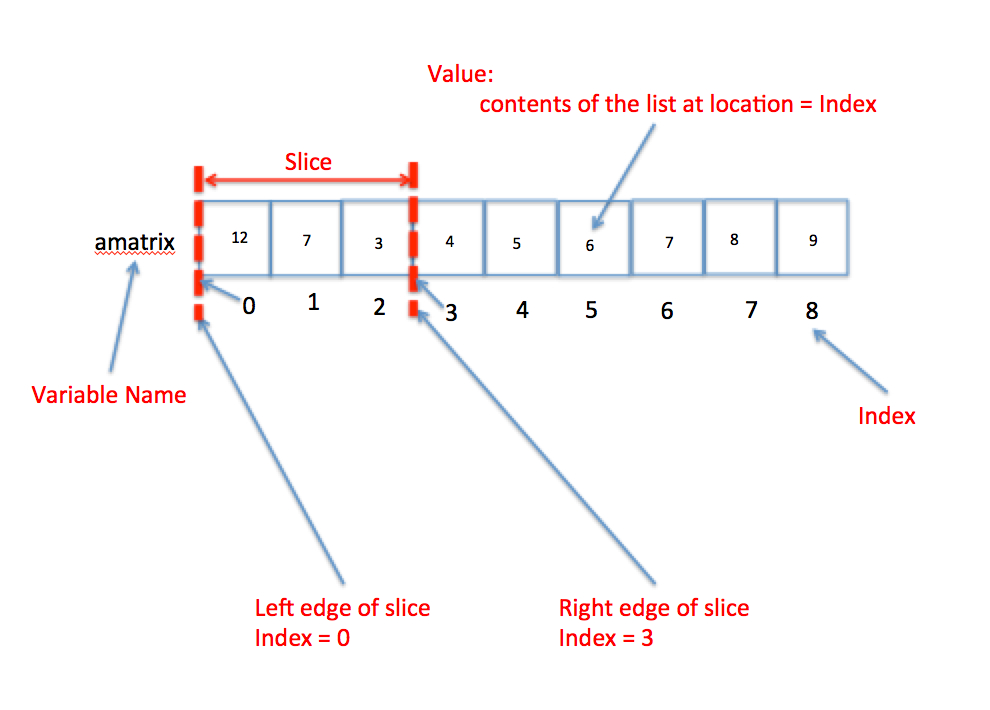
\includegraphics[width=6in]{./Matrix/SliceSchemeOne.jpg} 
%   \caption{Concept of slice from a list.}
%   \label{fig:SliceSchemeOne}
%\end{figure}
%
%So the index to the right of the left edge is the beginning of the slice, the index to the right of the right edge is the index of the end of the slice.  
%
%Alternatively we can simply say that Python addresses an index list from start to end, but does not actually get the end value, instead only end-1.  It's weird, but it is how the author of Python created the language.   FORTRAN has a similar weirdness in that it starts at 1 (rather than zero) for its counting scheme.
%
%Figure \ref{fig:SlicesAndMatrix} is a schematic of how slices and the row column structure of a matrix are conceptualized.   As far as the computer is concerned, a matrix is just a long list and we (humans) are the fools who invented this whole row column thing.   I find that if I think of the matrix as a vector with Z-folds at the column ends, I can deconstruct the single list into a set of lists, now indexed by row and column (just like I was taught in linear algebra forever ago).
%
%\begin{figure}[h!] %  figure placement: here, top, bottom, or page
%   \centering
%   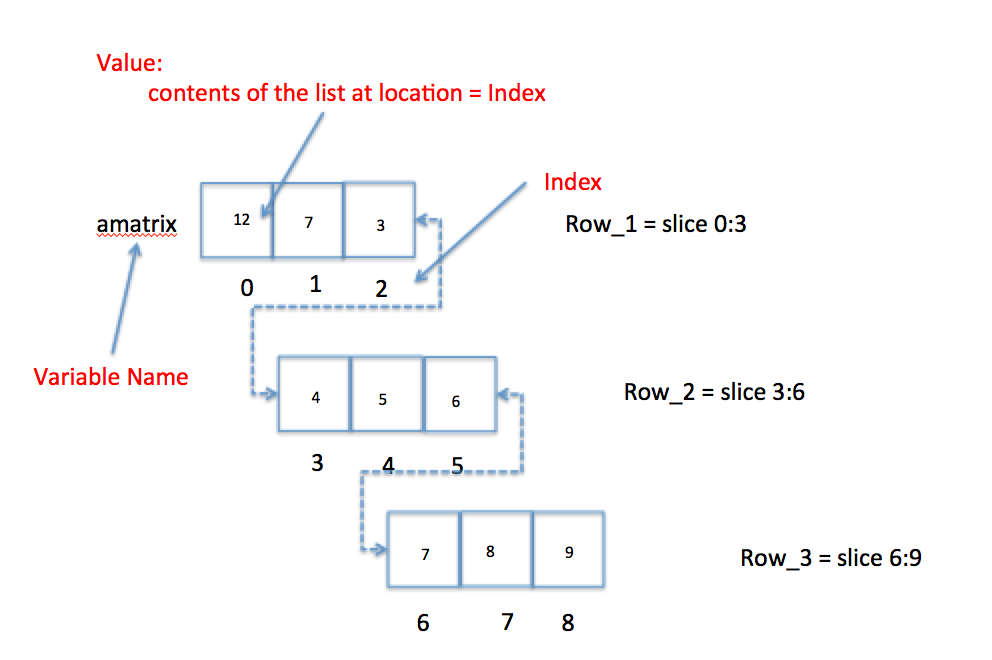
\includegraphics[width=6in]{./Matrix/SlicesAndMatrix.jpg} 
%   \caption{A conceptual diagram of slices and matrix relationships.  Each slice becomes a row.  We refer to an element by its row column index e.g. \texttt{amatrix[row][col]}. }
%   \label{fig:SlicesAndMatrix}
%\end{figure}

But this simply won't work because lists while they can contain floats, are not themselves floats -- the are lists.  So the above code which would be super natural in FORTRAN, C++, BASIC, ALGOL, PASCAL, RUBY, is useless in Python.  

However the following works quite nicely
\begin{verbatim}
amatrix[:] = [value * MyScalar for value in amatrix]
\end{verbatim}

